 
\section{Air Quality Sensors}
\label{sec:implementation_aqs}

\subsubsection*{London}

London is one of the cities that are available in the iCity platform. The city
of London has three services integrated in iCity:

\begin{enumerate}
  \itemsep0em
  \item {\bf Air Quality Sensors}. This service has sensors deployed all across
the city of London. These sensors mesure the air quality of the city. More
specifically, these sensors send data about the levels of: $NO_2$, SO, $O_3$,
PM10 and PM25.
  \item {\bf TFL Journey Planner}. This service gives access to developers to
the TFL API.
  \item {\bf Alert ME}. This platform is a Smart Home platform.
\end{enumerate}

The second and the third points are not really interesting in our case because
we need a source that is public and that sends data constantly. Therefore, for
this project I have picked the Air Quality Sensors platform.

\subsubsection*{Design and implementation}

Even if the Air Quality Sensors platform (AQS from now on) is the most complete
service from London, it has some major drawbacks:

\mylist
  \item The {\bf update rate} is low. Apparently the sensors from this platform
send data every hour. Nothing more, nothing less. This is quite frankly, a
poor update rate.
  \item There are lots of sensors that are not working. I have found that a lot
of the deployed sensors are not working at all.
\mylistend

Because of my points above, I have decided that I will not provide a streaming
API around this platform. Instead, I have built a minimal API around this
platform that only wraps up the API to provide some extra information.

The Storm application implements support for this platform through the {\bf
com.mssola.snacker.aqs} Scala package. This package is located in the
``snacker-aqs'' directory. The topology of this package is the following:

\begin{center}
  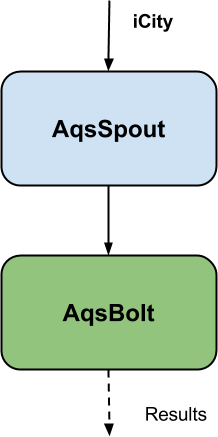
\includegraphics[scale=0.6]{implementation/images/aqs.png}
\end{center}

\begin{itemize}
  \itemsep0em
  \item The {\bf AqsSpout} is the only spout for this platform. This spout
fetches the data from iCity. After fetching it, this spout cleans and sends the
data to the AqsBolt.
  \item The {\bf AqsBolt} is the only bolt for this platform. This bolt
receives the data from the AqsSpout. After this, it performs some computations
and sends the results through a socket.
\end{itemize}

As I have previously said, this platform will not have a streaming API. This
means that when the API layer gets the data from the socket, it will close this
socket instantly. Therefore, the lifecycle of an HTTP request follows these
steps:

\begin{enumerate}
  \itemsep0em
  \item The API layer receives an HTTP request that points to the AQS service.
  \item The API layer subscribes to the AQS service for this request.
  \item The AQS module computes the results and sends them through the socket.
  \item The API layer receives the data and unsubscribes this request from AQS.
  \item The API layer generates a response with the given data.
\end{enumerate}

\subsubsection*{API endpoints}

The API for this service is minimal: I have implemented only one endpoint. This
is because the AQS service is really simple, and there are not a lot of
options here. This is the endpoint for this service:

\begin{center}
  /aqs/\{id\}/interval
\end{center}

The {\bf id} parameter has two possible values: ``all'' or a device id. The
possibility of getting the value for all the devices in a single request is
huge step forward in comparison of the iCity API. Besides the ``id'' parameter,
the developer has to include the following parameters in the request:

\mylist
  \item The {\bf from} and the {\bf to} parameters. These parameters are UNIX
timestapmps containing the interval of time.
  \item The {\bf property} parameter. Possible values are: ``no2'', ``so'',
``o3'', ``pm10'' and ``pm25''.
\mylistend

Calling this endpoint will result in a JSON response containing the values for
the specified properties and devices.
